%$Header: /cvsroot/latex-beamer/latex-beamer/solutions/generic-talks/generic-ornate-15min-45min.en.tex,v 1.4 2004/10/07 20:53:08 tantau Exp $
\documentclass{beamer}
\mode<presentation>
{
  \usecolortheme{seahorse}
  \usefonttheme{professionalfonts}
  \useinnertheme{rounded}
  \useoutertheme{shadow}
%  \useoutertheme{smoothbars}
}
%\setbeamertemplate{background canvas}[vertical shading][bottom=white!10,top=blue!5]
\usepackage{verbatim} 
\usepackage[english]{babel}
\usepackage[latin1]{inputenc}
\usepackage{pgf,pgfarrows,pgfnodes,pgfautomata,pgfheaps,pgfshade}
\usepackage{amsmath,amsfonts,amsthm,amssymb}
\usepackage{times}
\usepackage[T1]{fontenc}
\usepackage{graphics}
\usepackage{graphicx}
%\usepackage{psfig}
\usepackage{algorithmic}

\title
{Scilab based Mini Circuit Simulator for Academic Purpose}

\author[]
{Yogesh Dilip Save}
\institute
{
  Indian Institute of Technology, Bombay
}
%\pgfdeclareimage[height=0.7cm]{university-logo}{iitblogo.eps}
%\logo{\pgfuseimage{university-logo}}


\date[seminar] % (optional)
{\today}


\begin{document}
%***************************************************************************************
\begin{frame}
  \titlepage
\end{frame}
%***************************************************************************************
\begin{frame}
  \frametitle{Presentation Outline}
  \tableofcontents
\end{frame}
%***************************************************************************************

\section{Introduction}
\begin{frame}
 \frametitle{Motivation}
\begin{block}{Objective}
To assist students in improving their knowledge in field of circuit simulation.
\end{block}
\begin{block}{Problem with commercial simulators}
\begin{itemize}
\item Generally software codes are not available.
\item Software codes are written in higher level language (C Programming and Fortran....).
\item Complex due to implementation of many features and complex modeling.
\end{itemize}
\end{block}
\end{frame}

\begin{frame}
 \frametitle{Motivation}
\begin{block}{Objective}
To assist students in improving their knowledge in field of circuit simulation.
\end{block}
\begin{block}{Mini simulator}
\begin{itemize}
\item used Scilab for coding.
\item integrated least number of component.  
\item different versions for add-on features. 
\end{itemize} 
\end{block}
\end{frame}

\begin{frame}
 \frametitle{Plan}
\begin{block}{Display Symbolic Equations}
\end{block}
\begin{block}{Display Numerical Values}
\end{block}
\begin{block}{Complete Report Generation}
\end{block}
\begin{block}{GUI for circuit drawing}
\end{block}
\begin{block}{GUI for simulator option}
\end{block}
\begin{block}{Spoken Tutorial}
\end{block}
%\begin{block}
%\begin{itemize}
%\item Display Numerical Values  
%\item Complete Report Generation
%\item Graphical User Interface
%\item Spoken Tutorial 
%\end{itemize} 
%\end{block}
\end{frame}

\begin{frame}
 \frametitle{Core of circuit simulator}
\begin{itemize}
\item Operating Point Analysis plays an important role in a circuit simulation. 
\item DC Analysis is equivalent to performing OP Analysis at each voltages/currents. 
\item Transient Analysis is equivalent to performing OP Analysis at each time step.  
\item AC Analysis computes the small-signal behavior of a circuit about an operating point 
\item Thus implementation of Operating Point Analysis affects overall performance of the circuit simulator.
\end{itemize} 
\end{frame}

\section{Operating Point Analysis}
\begin{frame}
\begin{block}{Operating Point (OP) Analysis}
\begin{itemize}
\item OP Analysis is the central part of a circuit simulator.
\item The equations that describe the electrical system are nonlinear and algebraic and their solution gives operating point.
\item Systems of nonlinear equations are solved by iteratively formulating and solving systems of linear algebraic equations. 
\item The overall efficiency of a circuit simulator is dependent upon the performance of the linear DC analyzer.
%\item Thus, our work is towards improving the performance of linear DC Analyzers and handling convergence issues related to large size nonlinear circuits.
\end{itemize}
\end{block}
\end{frame}

\begin{frame}
\begin{block}{Circuit with linear elements}
\end{block}
\end{frame}

\begin{frame}
\begin{block}{\small Nodal Analysis}
\begin{itemize}
\begin{small}
\item Applicable when the network has only current sources and conductances type devices i.e., $i=g(v)$.
\item Let, $\mathbf{A}_r$ be the reduced incidence matrix of $\cal{G}$ which is a representative matrix of $V_v(\cal{G})$. \\
\end{small}
\begin{tiny}
The KCL constraints are
$$\mathbf{A_ri}=\mathbf{0}$$
$$\left[\begin{array}{cc}
  \mathbf{A}_{rG} & \mathbf{A}_{rJ}
\end{array}\right]
\left[\begin{array}{c}
  \mathbf{i}_{G} \\
  \mathbf{i}_{J}
\end{array}\right]
=\mathbf{0}$$
$$\mathbf{A}_{rG}\mathbf{i}_{G}=-\mathbf{A}_{rJ}\mathbf{i}_{J}$$

$$\mathbf{A}_{rG}\mathbf{G}\mathbf{v}_{G}=-\mathbf{A}_{rJ}\mathbf{i}_{J}\ \ \ \ \ \ \ \ (As, \mathbf{i}_{G}=\mathbf{G}\mathbf{v}_{G})$$

The KVE constraints are
$$\left[\begin{array}{c}
  \mathbf{v}_{G} \\
  \mathbf{v}_{J}
\end{array}\right]
=
\left[\begin{array}{c}
  \mathbf{A}_{rG}^T \\
  \mathbf{A}_{rJ}^T
\end{array}\right]
\mathbf{v}_n$$

\begin{equation}
\mathbf{A}_{rG}\mathbf{G}\mathbf{A}_{rG}^{T}\mathbf{v}_{n}=-\mathbf{A}_{rJ}\mathbf{i}_{J}
\label{nodal_equation}
\end{equation}
\end{tiny}
\end{itemize}
\end{block}
\end{frame}

\begin{frame}[fragile]
\begin{block}{Matrix Formulation}
\begin{itemize}
\item The diagonal entries of the matrix are the sum of conductances incident on the corresponding nodes.
\item The off diagonal entries $(i,j)^{th}$ of the matrix is the negative of conductances between node $i$ and $j$.
\item The $\mathbf{A}_{rJ}\mathbf{i}_{J}$ is the sum of current sources leaving the nodes.
\end{itemize}
\end{block}
\begin{block}{Example}
\end{block}
\begin{minipage}[!b]{0.4\linewidth} % A minipage that covers half the page
\begin{figure}[h]
\centering
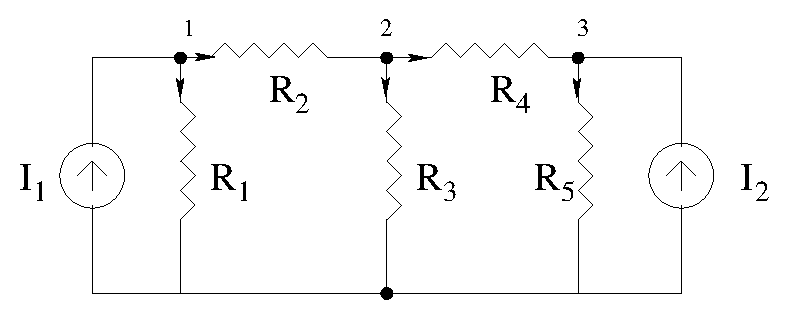
\includegraphics[scale=0.35]{../figures/nodal_figure.eps}
\end{figure}
\end{minipage}
\begin{minipage}[!b]{0.55\linewidth} % A minipage that covers half the page
\begin{tiny}
$$\left[
\begin{array}{ccc}
\widehat{R}_{1}+\widehat{R}_{2} & -\widehat{R}_{2} & 0\\
-\widehat{R}_{2} & \widehat{R}_{2}+\widehat{R}_{3}+\widehat{R}_{4} & -\widehat{R}_{4}\\
0 & -\widehat{R}_{4} & \widehat{R}_{4}+\widehat{R}_{5}
\end{array}
\right] \left[
\begin{array}{c}
v_{1}\\
v_{2}\\
v_{3}
\end{array}
\right]= \left[
\begin{array}{c}
I_{1}\\
0\\
I_{2}
\end{array}
\right]$$
\end{tiny}
\end{minipage}
\tiny $$\mbox{Note that } \widehat{R}=1/R$$
\tiny \href{run:../../LPCSim_1.0/ckt/nodalExample.ckt}{\color{red} Click here to see the example}
\end{frame}


\begin{frame}
\begin{block}{Modified Nodal Analysis}
\begin{small}
\begin{itemize}
\item applicable to all kinds of networks.
\item Let $\mathbf{A}_{r}$ be the reduced incidence matrix of ${\cal{G}}$
By Tellegan's theorem,
\begin{tiny}
$$\mathbf{A_ri}=\mathbf{0}$$
$$\left[\begin{array}{ccc}
  \mathbf{A}_{rG} & \mathbf{A}_{rT} & \mathbf{A}_{rJ}
\end{array}\right]
\left[\begin{array}{c}
  \mathbf{i}_{G} \\
  \mathbf{i}_{T} \\
  \mathbf{i}_{J}
\end{array}\right]
=\mathbf{0}$$

$$\left[\begin{array}{cc}
  \mathbf{A}_{rG}\mathbf{G} & \mathbf{A}_{rT}
\end{array}\right]
\left[\begin{array}{c}
  \mathbf{v}_{G} \\
  \mathbf{i}_{T}
\end{array}\right]
=-\mathbf{A}_{rJ}\mathbf{i}_{J}$$

\begin{equation}
\label{mna_eq1}
\left[\begin{array}{cc}
  \mathbf{A}_{rG}\mathbf{G}\mathbf{A}_{rG}^{T} & \mathbf{A}_{rT}
\end{array}\right]
\left[\begin{array}{c}
  \mathbf{v}_{n} \\
  \mathbf{i}_{T}
\end{array}\right]
=-\mathbf{A}_{rJ}\mathbf{i}_{J}
\end{equation}

Device characteristics of the branches in $T$ be
$$\left[\begin{array}{cc}
  \mathbf{M} & \mathbf{N}
\end{array}\right]
\left[\begin{array}{c}
  \mathbf{i}_{T} \\
  \mathbf{v}_{T}
\end{array}\right]
=\mathbf{S}_{T}$$

\begin{equation}
\label{mna_eq2}
\left[\begin{array}{cc}
  \mathbf{NA}_{rT}^{T} & \mathbf{M}
\end{array}\right]
\left[\begin{array}{c}
  \mathbf{v}_{n} \\
  \mathbf{i}_{T}
\end{array}\right]
=\mathbf{S}_{T}
\end{equation}
\end{tiny}
\end{itemize}
\end{small}
\end{block}
\end{frame}

\begin{frame}
\begin{block}{Example}
\begin{figure}[!ht]
\begin{center}
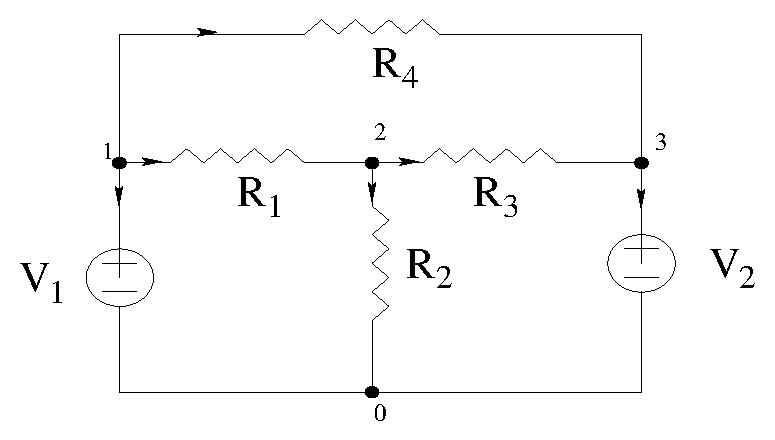
\includegraphics[scale=0.35]{../figures/modified_figure.eps}
\caption{ Example for MNA } \label{modifiedfig}
\end{center}
\end{figure}
\begin{tiny}
$$\left[
\begin{array}{cccccc}
\widehat{R}_{1}+\widehat{R}_{4} & -\widehat{R}_{1} & -\widehat{R}_{4} & 1 & 0 \\
-\widehat{R}_{1} & \widehat{R}_{1}+\widehat{R}_{2}+\widehat{R}_{3} & -\widehat{R}_{3} & 0 & 0 \\
-\widehat{R}_{4} & -\widehat{R}_{3} & \widehat{R}_{3}+\widehat{R}_{4} & 0 & 1  \\
1 & 0 & 0 & 0 & 0 \\
0 & 0 & 1 & 0 & 0
\end{array}
\right] \left[
\begin{array}{c}
v_{1}\\
v_{2}\\
v_{3}\\
i_{V_1}\\
i_{V_2}\\
\end{array}
\right]= \left[
\begin{array}{c}
0\\
0\\
0\\
V_{1}\\
V_{2}
\end{array}
\right]$$
\end{tiny}
\tiny $$\mbox{Note that } \widehat{R}=1/R$$
\tiny \href{run:../../LPCSim_1.0/ckt/modifiedNodalExample.ckt}{\color{red} Click here to see the example}
\end{block}
\end{frame}

\begin{frame}
\frametitle{Controlled Sources}
\begin{minipage}[!b]{0.47\linewidth} % A minipage that covers half the page
  \begin{figure}[!ht]
      \centering
      
\includegraphics[scale=0.6]{../figures/VCCS.eps}
      \caption{\scriptsize Voltage Controlled Current Source (VCCS)}
      \label{vccs}
  \end{figure}
\end{minipage}
%\hspace{0.5cm} % To get a little bit of space between the figures
\begin{minipage}[!b]{0.47\linewidth}
  \begin{figure}[!ht]
     \centering
      
\includegraphics[scale=0.6]{../figures/VCVS.eps}
      \caption{\scriptsize Voltage Controlled Voltage Source (VCVS) }
      \label{vcvs}
  \end{figure}
    \end{minipage}
\begin{minipage}[!b]{0.47\linewidth} % A minipage that covers half the page
  \begin{figure}[!ht]
      \centering
      
\includegraphics[scale=0.6]{../figures/CCCS.eps}
      \caption{\scriptsize Current Controlled Current Source (CCCS)}
      \label{cccs}
  \end{figure}
\end{minipage}
%\hspace{0.5cm} % To get a little bit of space between the figures
\begin{minipage}[!b]{0.47\linewidth}
  \begin{figure}[!ht]
     \centering
      
\includegraphics[scale=0.6]{../figures/CCVS.eps}
      \caption{\scriptsize Current Controlled Voltage Source (CCVS) }
      \label{ccvs}
  \end{figure}
    \end{minipage}
\begin{scriptsize}
\begin{itemize}
\item In voltage controlled devices, we have added a $0A$ current source as controlling branch
%without disturbing the incidence relationship of existing edges (i.e., the addition is 'soldering type') and its voltage is used for calculating the value of the devices.
\item In current controlled devices, we have added a $0V$ voltage source as controlling branch
%by splitting a node (i.e., plier type entry) and the current through it is used for calculating the value of the devices.
\end{itemize}
\end{scriptsize}
\end{frame}

\begin{frame}
\begin{block}{Example with controlled sources}
\begin{figure}[!ht]
\begin{center}

\includegraphics[scale=0.6]{../figures/linearckt.eps}
\caption{ \scriptsize Example with controlled source (MNA)} \label{modifiedfig}
\end{center}
\end{figure}
\begin{tiny}
$$\left[
\begin{array}{ccccccc}
\widehat{R}_{1} & -\widehat{R}_{1} & 0 & 0 & 0 & 1 & 0 \\
-\widehat{R}_{1} & \widehat{R}_{1}+\widehat{R}_{2} & 0 & 0 & 0 & 0 &1\\
0 & 0& \widehat{R}_{4} & -\widehat{R}_{4}-g_1 & 0 & 0 & -1  \\
0 & 0& -\widehat{R}_{4} & \widehat{R}_{3}+ \widehat{R}_{4}+\widehat{R}_{5} &-\widehat{R}_{5}  & 0 & 0  \\
0 & 0& 0 &g_1-\widehat{R}_{5} & \widehat{R}_{5}+\widehat{R}_{6} & 0 & 0   \\
1 & 0 & 0 & 0 & 0 &0 &0\\
0 & 1 & -1 &-e1 &e1 &0 & 0
\end{array}
\right] \left[
\begin{array}{c}
v_{1}\\
v_{2}\\
v_{3}\\
v_{4}\\
v_{5}\\
i_{V_1}\\
i_{E_1}\\
\end{array}
\right]= \left[
\begin{array}{c}
0\\
0\\
I_1\\
0\\
0\\
V_{1}\\
0
\end{array}
\right]$$
\end{tiny}
\tiny $$\mbox{Note that } \widehat{R}=1/R$$
\tiny \href{run:../../LPCSim_1.0/ckt/linear1.ckt}{\color{red} Click here to see the example}
\end{block}
\end{frame}

\begin{frame}
\begin{block}{Example with controlled sources-2}
\begin{figure}[!ht]
\begin{center}

\includegraphics[scale=0.6]{../figures/linearckt2.eps}
\caption{ \scriptsize Example2 with controlled source (MNA)} \label{modifiedfig}
\end{center}
\end{figure}
\begin{tiny}
$$\left[
\begin{array}{cccccc}
\widehat{R}_{1}+\widehat{R}_{2} & -\widehat{R}_{2} & 0 & 0 & 0 &0\\
-\widehat{R}_{2} &\widehat{R}_{2}+\widehat{R}_{4} &0& -\widehat{R}_{4} & 1 & 0  \\
0 & -\widehat{R}_{4} & 0 & \widehat{R}_{4} & 0  & 1  \\
0 & 1& -1 &0 & 0 & 0   \\
0 & 0 & 0 & 1 & -h_1 &0 
\end{array}
\right] \left[
\begin{array}{c}
v_{1}\\
v_{2}\\
v_{3}\\
v_{4}\\
i_{V_1}\\
i_{H_1}\\
\end{array}
\right]= \left[
\begin{array}{c}
I_1\\
0\\
0\\
0\\
V_{1}\\
0
\end{array}
\right]$$
\end{tiny}
\tiny $$\mbox{Note that } \widehat{R}=1/R$$
\tiny \href{run:../../LPCSim_1.0/ckt/linear2.ckt}{\color{red} Click here to see the example}
\end{block}
\end{frame}

\begin{frame}
\frametitle{Circuit with nonlinear elements}
Simulation of circuit with nonlinear element is done in two steps:
\begin{itemize}
\item Formulating the nonlinear equilibrium equations using topological constraints (i.e., KCE, KVE).
\item Solving these equations using appropriate numerical technique.
\end{itemize} 
Newton-Raphson method -- Numerical technique to solve nonlinear equations
\begin{itemize}
\item fast convergence rate
\item needs good initial guess
\item does not guaranteed to converge
\item slower when multiple solution
\end{itemize}
\end{frame}

\begin{frame}
\frametitle{Linearization of Nonlinear Elements}
\begin{minipage}[!b]{0.5\linewidth}
Diode characteristics,
$$I_D=I_S(e^{qV/kT}-1)$$
$$I_D=I_D|_{V=V_0} + (V-V_0)\frac{I_D}{V}|_{V=V_0}$$
$$I_D=I_{D0}+(V-V_0)G_{D0}$$
\begin{figure}[h]
\begin{center}
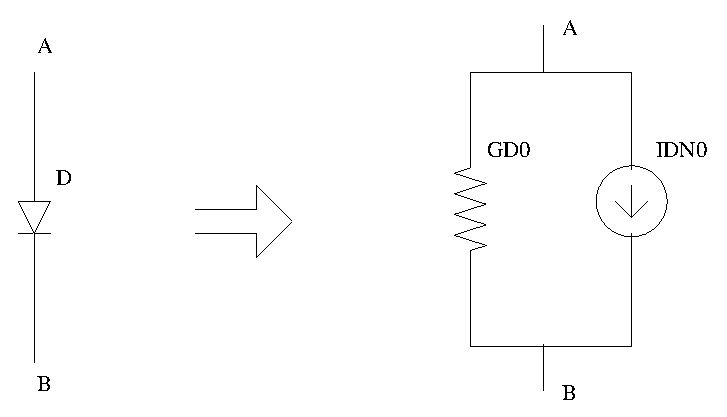
\includegraphics[scale=0.4]{../figures/diodeI.eps}
\begin{small}Modeling of Diode\end{small}
\label{diodeI}
\end{center}
\end{figure}
\end{minipage}
\begin{minipage}[!b]{0.4\linewidth}
\begin{figure}[h]
\begin{center}
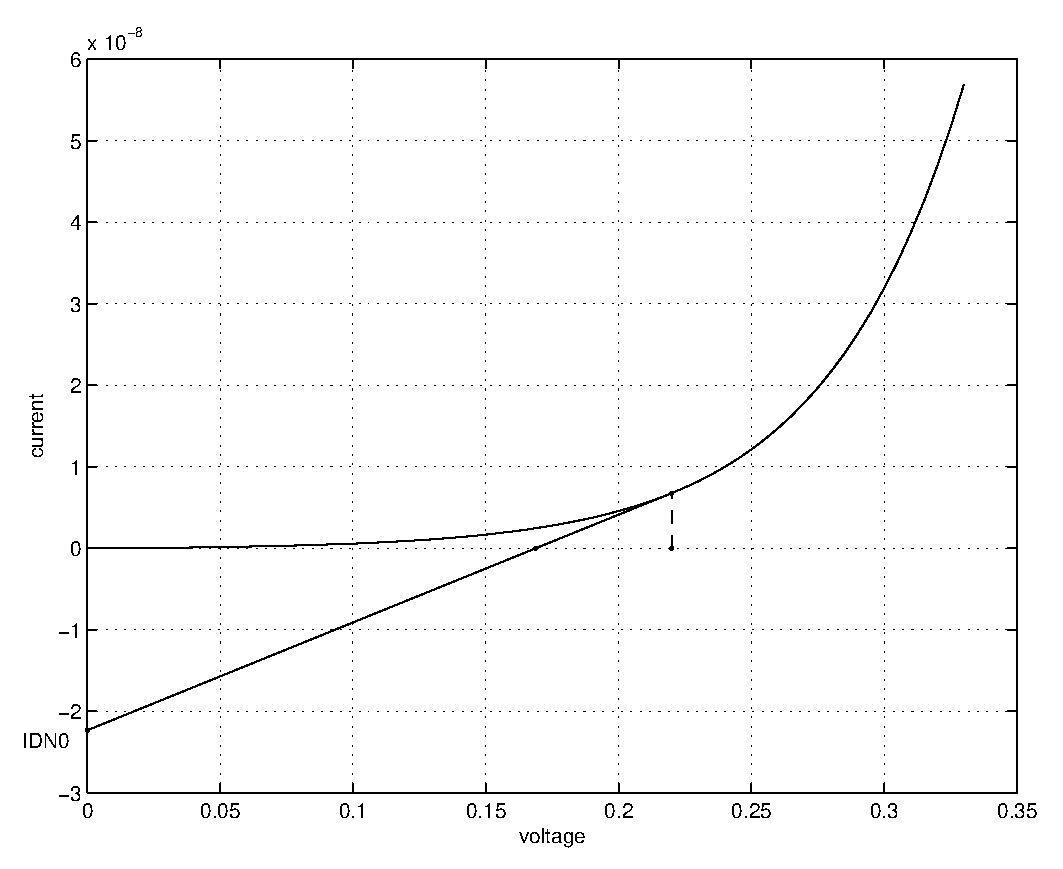
\includegraphics[scale=0.3]{../figures/diodechar1.eps}
\begin{small}Linearized approximation of diode model\end{small}
\begin{tiny}$$I_{DN0}=I_{D0}-V_0G_{D0}$$\end{tiny}
\end{center}
\end{figure}
\end{minipage}
\end{frame}


\begin{frame}
{\bf Procedure:}{Operating Point Analysis}
\small
\begin{algorithmic}[1]
\STATE Find Node Potential and Current through devices whose device characteristic can not be expressed in terms of voltage.
\STATE Find branch voltage and node potential.
\STATE Find branch current from branch voltage using device characteristics.
\IF{Non-linear component}
\STATE {\bf NR:} Check  device characteristics of non-linear devices.
\IF {Device characteristics is not satisfied}
\STATE Call Newton Raphson procedure
\STATE Find Node Potential and Current through devices whose device characteristic can not be expressed in terms of voltage.
\STATE Find branch current from branch voltage using device characteristics.
\STATE Go to {\bf NR}
\ENDIF
\STATE Check for KCL
\ENDIF
\end{algorithmic}
\normalsize
\end{frame}

\begin{frame}
\frametitle{Full Wave Bridge Rectifier}
\begin{minipage}[!b]{0.4\linewidth} % A minipage that covers half the page
\begin{figure}[h]
\centering
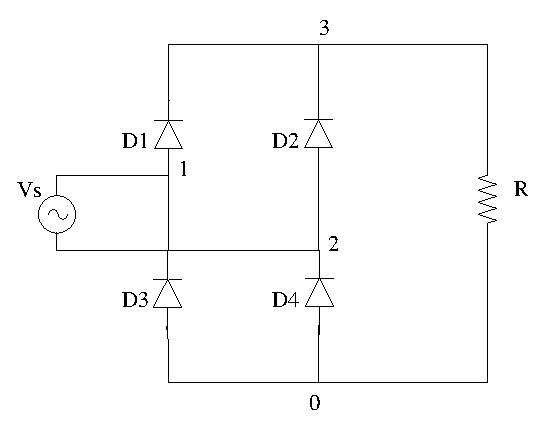
\includegraphics[scale=0.5]{../figures/bridge.eps}
\end{figure}
\end{minipage}
\hspace{0.5cm} % To get a little bit of space between the figures
\begin{minipage}[!b]{0.5\linewidth} % A minipage that covers half the page
\begin{figure}[h]
\centering
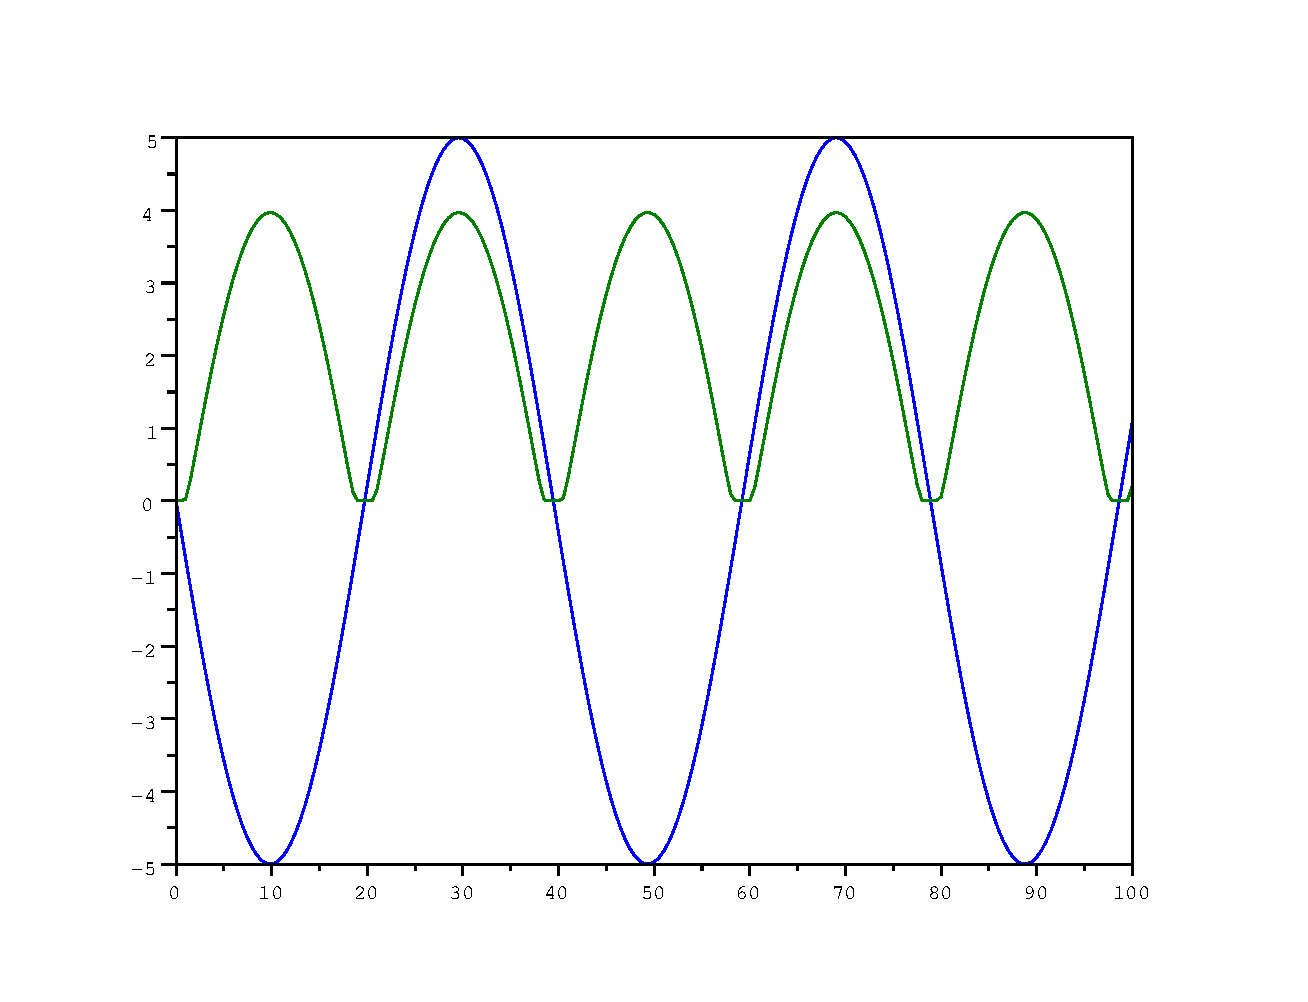
\includegraphics[scale=0.3]{../figures/bridgeOutput.eps}
\end{figure}
\end{minipage}
\end{frame}

\section{DC Analysis}
\begin{frame}
\frametitle{DC Analysis}
{\bf Procedure:}{DC Analysis}
\small
\begin{algorithmic}[1]
\STATE Modify the value of the sweep source and update Modified Nodal matrix.
\STATE Do Operating Point Analysis.
\end{algorithmic}
\normalsize
\end{frame}

\begin{frame}
\frametitle{Voltage Sweep}
\begin{minipage}[!b]{0.4\linewidth} % A minipage that covers half the page
\begin{figure}[h]
\centering
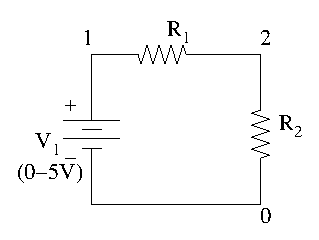
\includegraphics[scale=0.8]{../figures/V_Sweep.eps}
\caption{Example of DC Analysis (Vsweep.ckt)}
\end{figure}
\end{minipage}
\hspace{0.5cm} % To get a little bit of space between the figures
\begin{minipage}[!b]{0.5\linewidth} % A minipage that covers half the page
\begin{figure}[h]
\centering
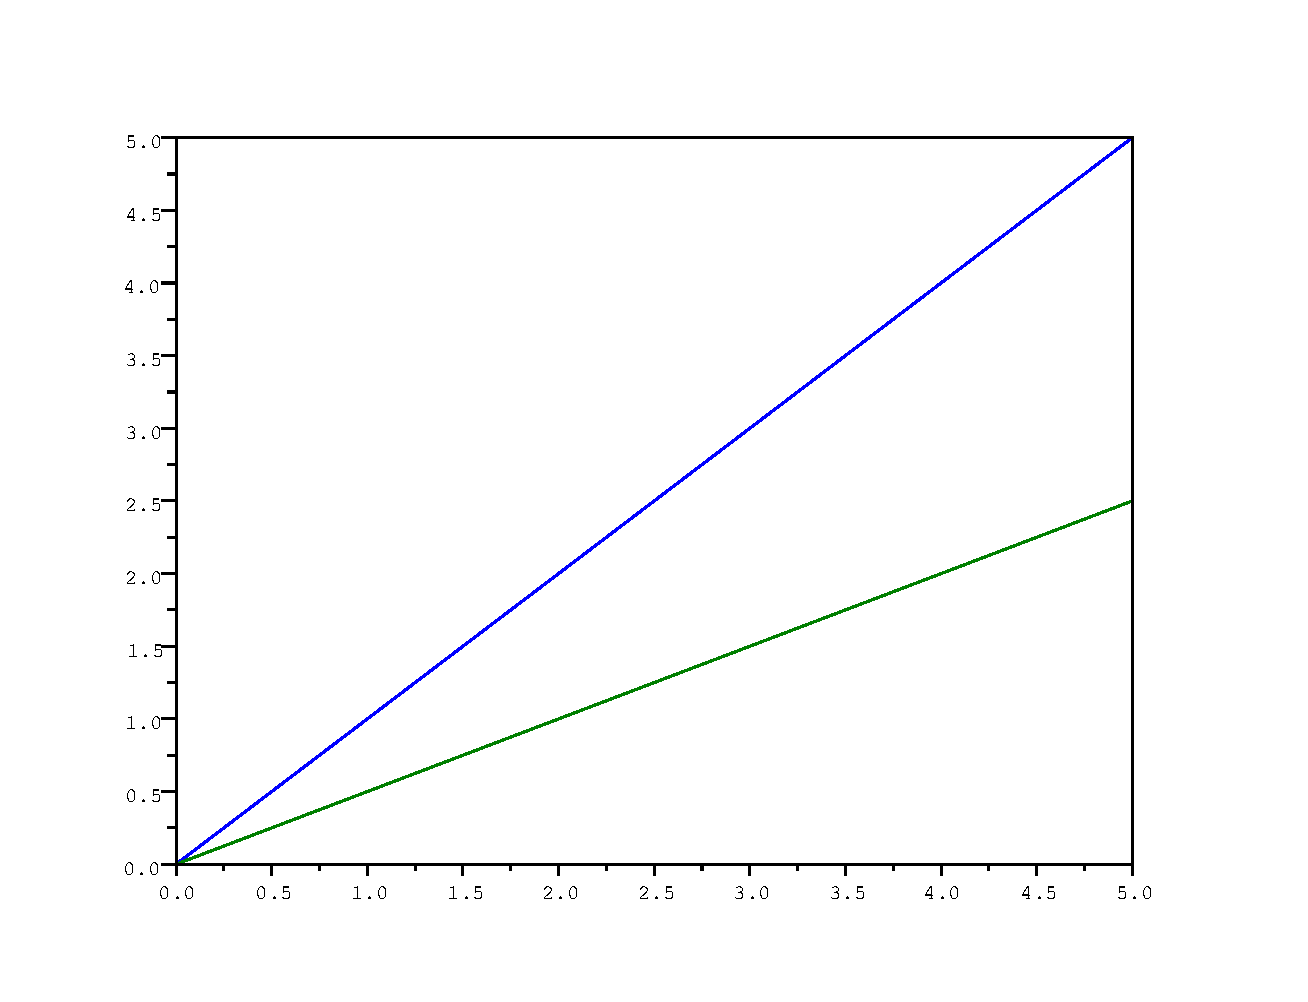
\includegraphics[scale=0.3]{../figures/V_SweepOutput.eps}
\end{figure}
\end{minipage}
\end{frame}

\begin{frame}
\frametitle{User defined Components}
Consider, a non-linear resistance,
$$I=\frac{1}{R}V^3$$

\begin{itemize}
\item Create  a file \$CompName.sci
\item Define
\begin{itemize}
\item Function in the $i=g(v)$ form
\item Jacobian of the function
\end{itemize}
\end{itemize}

%{\bf Syntax:-}
%\newline
%function I=\$CompName\_func(voltage,parameter)
%\$par\_2=parameter(2)
%\$par\_3=parameter(3)
\end{frame}

\begin{frame}
\frametitle{Non-linear Resistance}
\begin{minipage}[!b]{0.43\linewidth} % A minipage that covers half the page
\begin{figure}[h]
\centering
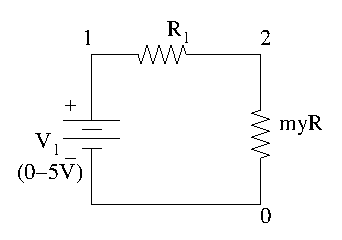
\includegraphics[scale=0.7]{../figures/myR.eps}
\end{figure}
\begin{tiny}
function I=myR\_func(voltage,parameter)
\begin{center}
        R=parameter(2); \newline
        I=1/R*(voltage\^3);
\end{center}
endfunction \newline


function Gj=myR\_Jacobian(voltage,parameter) 
\begin{center}
        R=parameter(2); \newline
        Gj=3/R*(voltage\^2);
\end{center}
endfunction
\end{tiny}
\end{minipage}
\hspace{0.5cm} % To get a little bit of space between the figures
\begin{minipage}[!b]{0.5\linewidth} % A minipage that covers half the page
\begin{figure}[h]
\centering
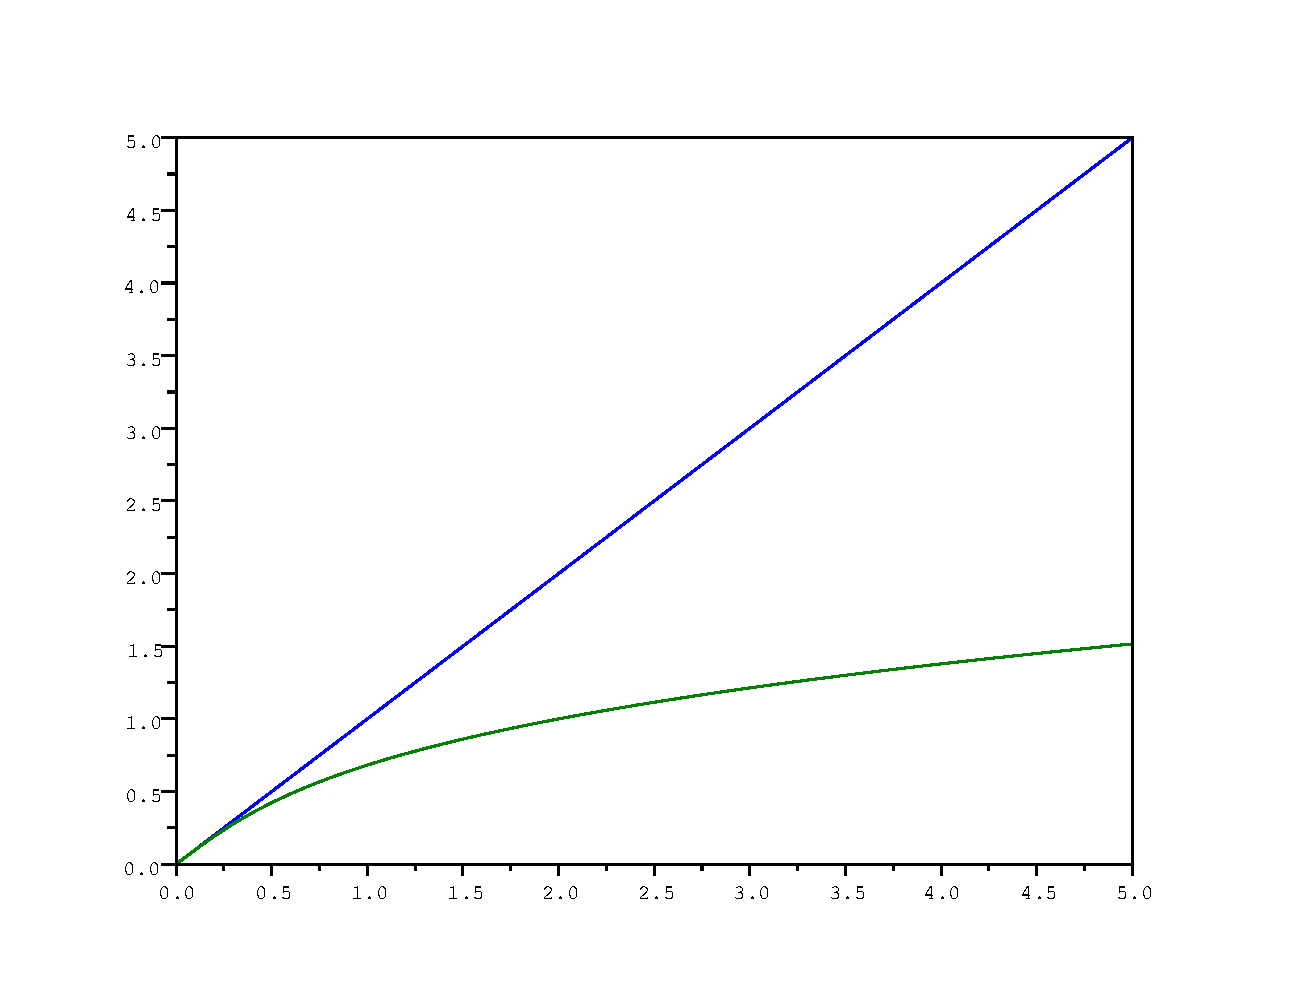
\includegraphics[scale=0.3]{../figures/myROutput.eps}
\end{figure}
\end{minipage}
\end{frame}

\section{Transient Analysis}
\begin{frame}
  \begin{block}{What is Transient Analysis?}
     \begin{itemize}
       \item Computes the response of a circuit as function of time.
       \item Time is discretized and the solution is computed piecewise.
     \end{itemize}
   \end{block}
  \begin{block}{Important factors}
    \begin{itemize}
      \item Proper time Stepping.
      \item Integration methods.
    \end{itemize}
  \end{block}
\end{frame}

\begin{frame}
\frametitle{Discreatization}
Consider, a capacitor
\begin{tiny}
$$I_C(t_n)=C\frac{\partial{V}_C(t_n)}{\partial{t}}$$
Using Backward Euler's method,
$$I_C(t_n)=C\frac{V(t_n)-V(t_{n-1})}{t_n-t_{n-1}}$$
$$I_C(t_n)=\frac{C}{h}V(t_n)-\frac{C}{h}V(t_{n-1})$$
$$I_C(t_n)=G_C^{(k)}V(t_n)-I_C^{(k)}$$
\end{tiny}
\begin{figure}[h]
\centering
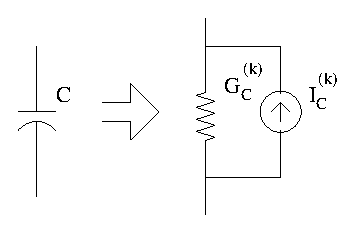
\includegraphics[scale=0.8]{../figures/Ceq.eps}
\end{figure}
\end{frame}

\begin{frame}
\frametitle{RC Circuit}
\begin{minipage}[!b]{0.4\linewidth} % A minipage that covers half the page
\begin{figure}[h]
\centering
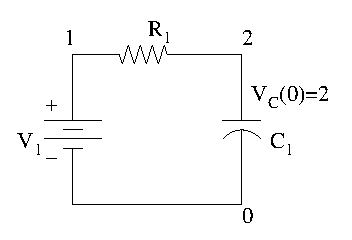
\includegraphics[scale=0.8]{../figures/RC.eps}
\end{figure}
\end{minipage}
\hspace{0.5cm} % To get a little bit of space between the figures
\begin{minipage}[!b]{0.5\linewidth} % A minipage that covers half the page
\begin{figure}[h]
\centering
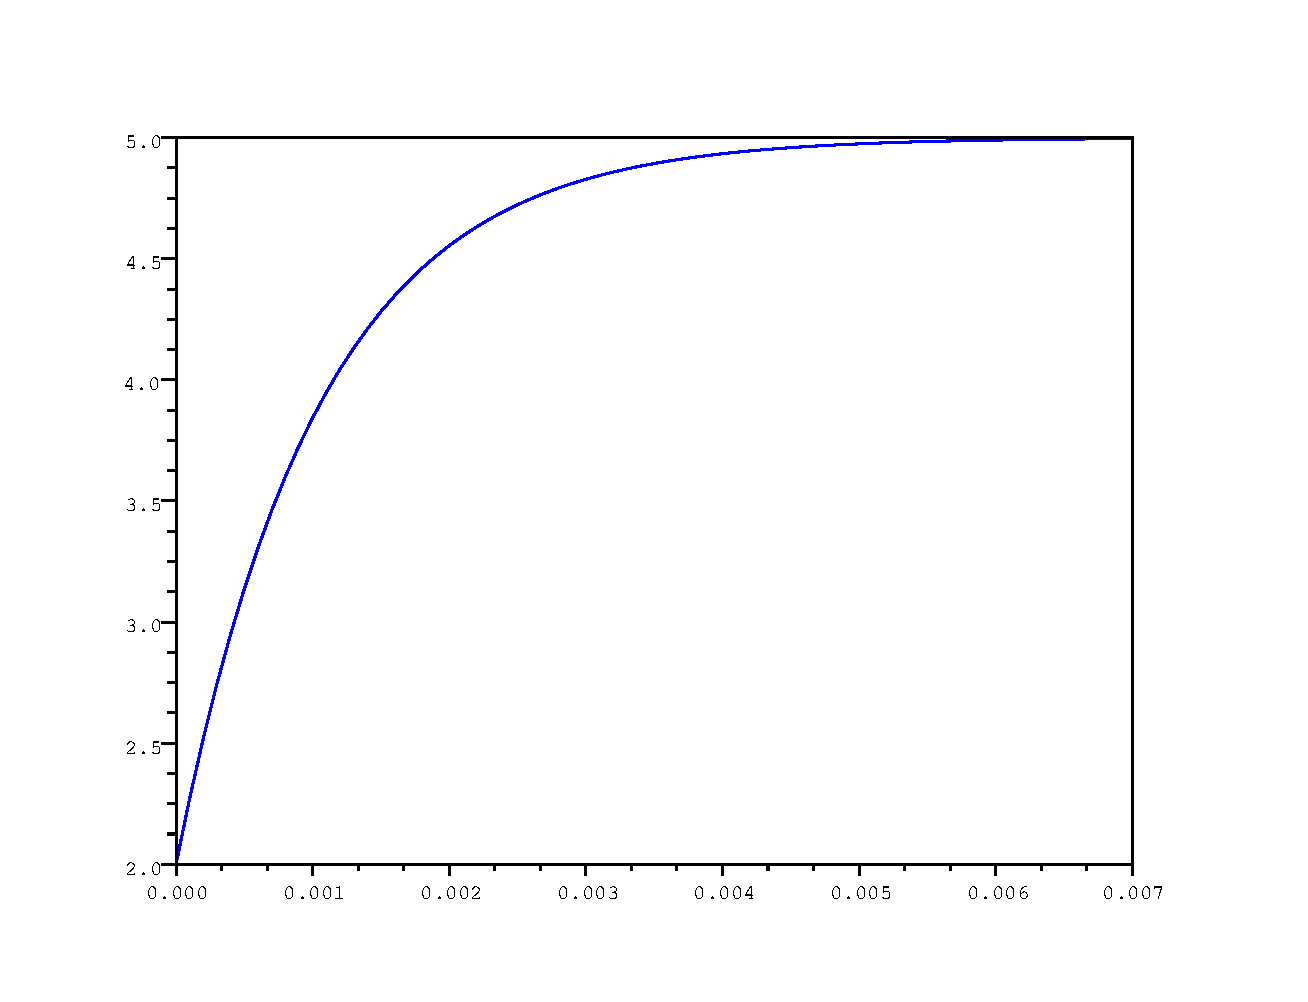
\includegraphics[scale=0.3]{../figures/RCOutput.eps}
\end{figure}
\end{minipage}
\end{frame}

\begin{frame}
\frametitle{Full Wave Bridge Rectifier with Filter}
\begin{minipage}[!b]{0.4\linewidth} % A minipage that covers half the page
\begin{figure}[h]
\centering
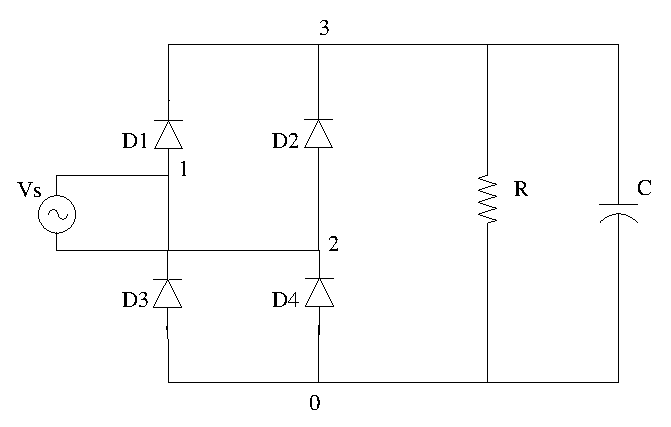
\includegraphics[scale=0.4]{../figures/bridgeFilter.eps}
\end{figure}
\end{minipage}
\hspace{0.5cm} % To get a little bit of space between the figures
\begin{minipage}[!b]{0.5\linewidth} % A minipage that covers half the page
\begin{figure}[h]
\centering
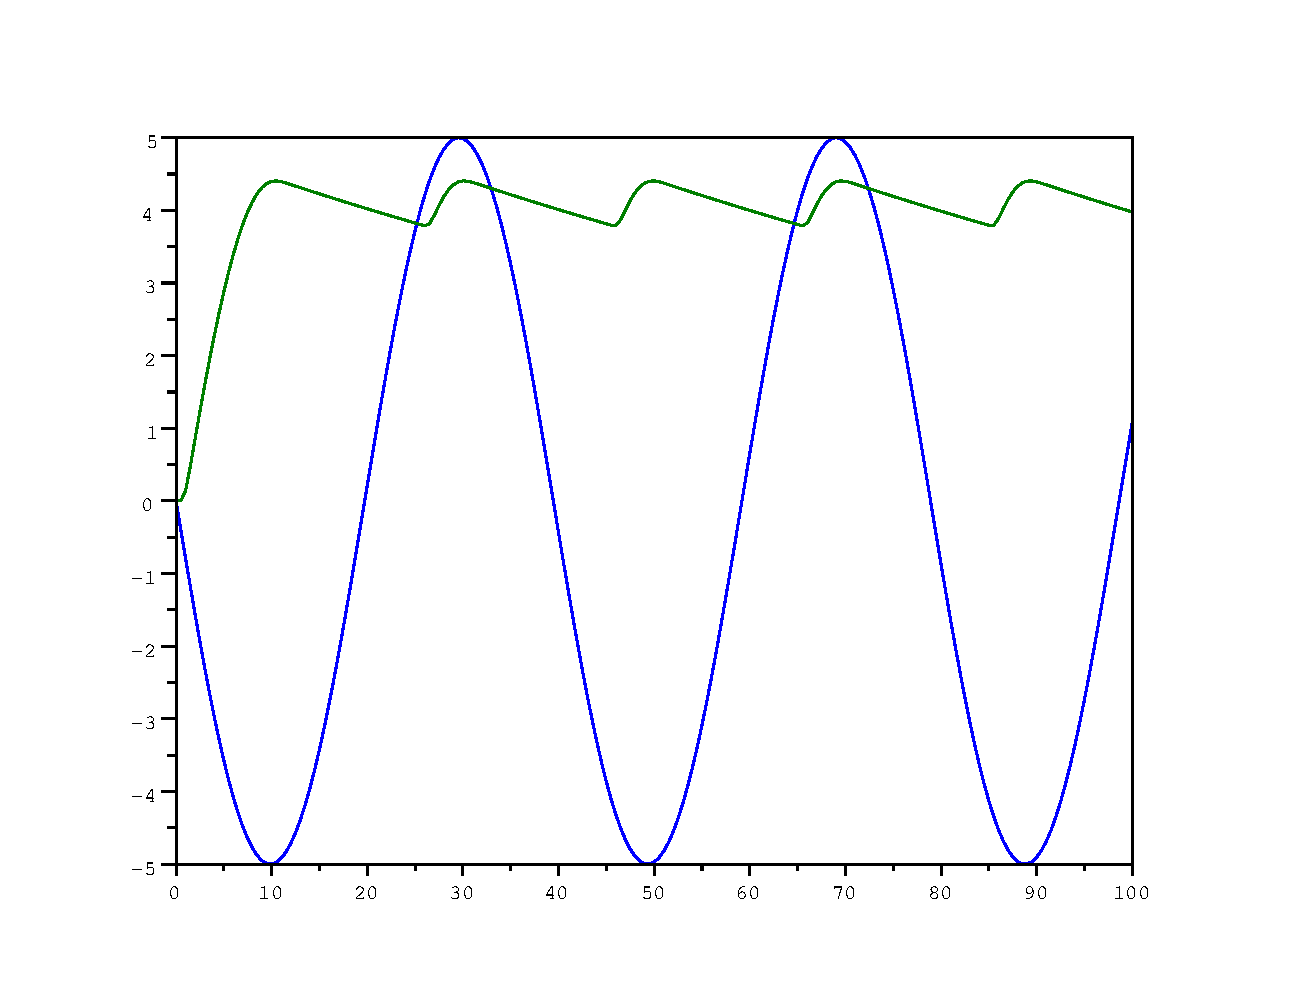
\includegraphics[scale=0.3]{../figures/bridgeFilterOutput.eps}
\end{figure}
\end{minipage}
\end{frame}

\begin{frame}
\frametitle{PseudoCode}
{\bf Procedure:}{Transient Analysis}
\small
\begin{algorithmic}[1]
\STATE Discretize time dependent Component and Update Modified Nodal matrix.
\STATE Do Operating Point Analysis.
\end{algorithmic}
\normalsize

{\bf Procedure:}{Discretization}
\small
\begin{algorithmic}[1]
\STATE Compute time dependent source value at time t.
\STATE Compute the values of static model of dynamic component at time t.
\STATE Update Modified Nodal matrix.
\end{algorithmic}
\normalsize
\end{frame}

%\begin{frame}
%\frametitle{CMOS Inverter}
%\begin{minipage}[!b]{0.4\linewidth} % A minipage that covers half the page
%\begin{figure}[h]
%\centering
%\includegraphics[scale=0.4]{../figures/inverter.eps}
%\end{figure}
%\end{minipage}
%\hspace{0.5cm} % To get a little bit of space between the figures
%\begin{minipage}[!b]{0.5\linewidth} % A minipage that covers half the page
%\begin{figure}[h]
%\centering
%\includegraphics[scale=0.3]{../figures/inverterOutput.eps}
%\end{figure}
%\end{minipage}
%\end{frame}

\end{document}

